\documentclass[11pt]{article}
% Use [review] for an anonymous submission with line numbers.
\usepackage[final]{acl}
\usepackage{times}
\usepackage{latexsym}
\usepackage{microtype}

\usepackage{amsmath,amssymb,amsfonts}
\usepackage{algorithmic}
\usepackage{graphicx}
\usepackage{textcomp}
\usepackage{xcolor}
\usepackage[utf8]{vietnam}
\usepackage[vietnamese, english]{babel}
\usepackage{booktabs}
\usepackage{tabularx}
\usepackage{array}
\usepackage{multirow}
\usepackage{url}
\def\BibTeX{{\rm B\kern-.05em{\sc i\kern-.025em b}\kern-.08em
    T\kern-.1667em\lower.7ex\hbox{E}\kern-.125emX}}

\newcommand{\envi}{EN$\rightarrow$VI}
\newcommand{\vien}{VI$\rightarrow$EN}

\begin{document}

\title{Rainbow Cookie at VLSP 2026: Small Models, Long Laws}

\author{Trần Đức Lâm, Lê Vân Anh, Phạm Thị Khánh Linh, Nguyễn Thị Hiền Trang \\
University of Engineering and Technology, \\
Vietnam National University, Hanoi, Vietnam \\
\texttt{\small tranduclam06@gmail.com, vananh9684@gmail.com} \\
\texttt{\small 24022385@vnu.edu.vn, 24022470@vnu.edu.vn}}

\maketitle

\begin{abstract}
We describe our system for the VLSP 2026 shared task on document-level English--Vietnamese legal machine translation with models below 3 billion parameters. The system combines LoRA adaptation of Hy-MT2-1.8B on a processed legal corpus with a structure-aware Markdown pipeline. Adjacent legal prose is translated in blocks to retain local context, while deterministic checks identify structural failures and trigger one recovery round. Length-based batching and a GPU repetition guard control inference cost. On the public test set, the submitted configuration obtains 70.87 BLEU for English-to-Vietnamese and 47.44 BLEU for Vietnamese-to-English, taking 2.0 and 1.4 hours with approximately 5~GB peak allocated GPU memory per direction on a T4. Development comparisons examine model adaptation and node grouping, providing practical evidence for combining domain-specific training with structured inference under the task's resource constraints.
\end{abstract}

\section{Introduction}
Legal machine translation (MT) must preserve specialised terminology, rights, obligations, conditions and exceptions. Document structure also matters: article numbers, nested clauses, tables and signature blocks carry information that should survive translation. Long legal documents make these requirements difficult to satisfy within a small model's context window.

The VLSP 2026 shared task addresses English--Vietnamese legal MT with models below 3 billion parameters, fully local inference and no external APIs~\cite{vlsp2026}. Evaluation considers translation quality, terminology correctness and consistency, legal accuracy, inference time and peak memory. We describe a system built around Hy-MT2-1.8B, adapted with LoRA~\cite{hu2022lora} and deployed through a Markdown-aware translation pipeline.

Our system has two main components: (1) a cleaned and extended legal corpus with document-based splitting, alignment review and text normalisation; and (2) a pipeline that groups adjacent prose, checks structural constraints, retries failed units and detects repetitive generation on the GPU. Experiments compare two base models, their pipeline variants and their fine-tuned variants. The largest observed gain comes from fine-tuning with the pipeline fixed; a development experiment also favours grouped translation over one-node requests. These are system-development comparisons, with limitations discussed in Section~\ref{sec:limitations}.

\section{Related Work}
\textbf{Translation models and resources.} ALMA adapts LLMs through monolingual and parallel-data fine-tuning~\cite{xu2024alma}, while Tower combines continued pre-training and instruction tuning~\cite{alves2024tower}. Hy-MT2 provides a 1.8B translation model supporting 33 languages~\cite{zheng2026hymt2}. For English--Vietnamese, PhoMT offers 3.02 million sentence pairs~\cite{doan2021phomt}, and MTet provides 4.2 million training pairs and EnViT5 models~\cite{ngo2022mtet}. Our training units instead follow the structure of the task's legal documents.

\textbf{Document-level and legal MT.} Context-aware MT targets discourse phenomena such as deixis, ellipsis and lexical cohesion~\cite{voita2019context}; document-level approaches are surveyed by \citet{maruf2021survey}, and \citet{wang2023docllm} study LLMs as document translators. Legal adaptation includes QLoRA tuning of IndicTrans2~\cite{singh2025indictrans2} and domain-specific tuning on EU legislation~\cite{lorini2026eu}. Our contribution is a practical system integrating legal-data adaptation with Markdown preservation and bounded recovery. Its repetition guard addresses a known generation failure~\cite{holtzman2020degeneration}, with a repetition penalty~\cite{keskar2019ctrl} used on the recovery path.

\section{Method}
The system combines legal-data preparation, LoRA fine-tuning and structured inference.

\subsection{Training Data Processing}\label{sec:data}
\begin{figure*}[t]
\centering
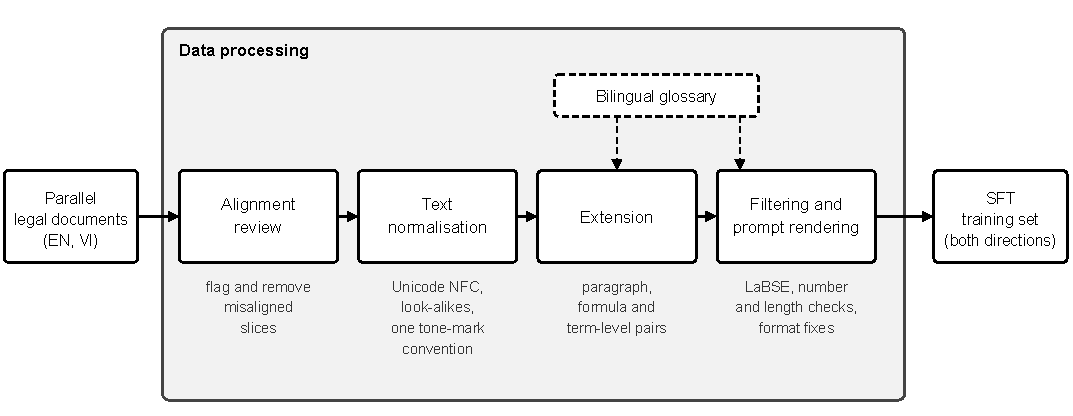
\includegraphics[width=\textwidth]{fig1.pdf}
\caption{Preparation of the supervised fine-tuning corpus.}
\label{fig:data}
\end{figure*}
Parallel Markdown documents are sliced at preamble, article, clause, adjacent-article and whole-document boundaries. A row pairs a slice with its translation. Processing (Fig.~\ref{fig:data}) expands the initial 54,134 rows from 575 training documents to 82,203 rows from 612 documents; the latter comprise 571 retained training documents and all 41 development documents, with four initial training documents absent after filtering. The final composition is given in Table~\ref{tab:composition}. All training data come from organiser-provided data or are written by the authors; we use no external parallel or monolingual corpora.

\textbf{Alignment review.} We flag 237 slices with inconsistent document codes or large numbers, exclude 158 after manual review, and propagate removals to slices containing the same erroneous segment. Flags require review because numbers may be written differently across languages.

\textbf{Text normalisation.} We normalise Unicode to NFC, repair look-alike and legacy characters, remove invisible characters and unify Vietnamese tone placement on \emph{oa}, \emph{oe} and \emph{uy}. The same normaliser processes inference sources.

\textbf{Glossary and data split.} A glossary of 442 bilingual pairs supplies training hints in 19,495 of 82,203 rows (23.7\%). Co-occurrence in aligned training texts is checked automatically; this does not constitute a complete expert semantic review. Splitting is by document, keeping all slices together. The development split is later merged into training, while 23 documents held out from the task's training data (not among the 575) are used only for validation loss and a fixed fit check, never for training.

\textbf{Extension and filtering.} We add paragraph pairs, hand-written legal formula phrases and terminology pairs (Table~\ref{tab:composition}). Further filtering uses LaBSE similarity on flagged pairs~\cite{feng2022labse}, length ratios, national-title consistency, amounts and list labels. Manual edits correct residual OCR/typing errors and standardise thousands separators and fine-amount expressions.

\begin{table}[t]
\centering
\small
\begin{tabular}{lr}
\toprule
Component & Rows \\
\midrule
Original rows after cleaning & 50,129 \\
Paragraph-level rows & 30,658 \\
Hand-written formula rows & 654 \\
Terminology rows & 762 \\
\midrule
\textbf{Total} & \textbf{82,203} \\
\bottomrule
\end{tabular}
\caption{Composition of the final training data.}
\label{tab:composition}
\end{table}

\subsection{Base Models and Fine-Tuning}\label{sec:finetune}
We fine-tune Hy-MT2-1.8B~\cite{zheng2026hymt2} and Index-Translate-2B~\cite{indexteam} on the processed corpus, freezing base weights and learning LoRA matrices in attention and MLP projections. Hy-MT2 uses two consecutive training passes; configurations are summarised in Appendix~\ref{app:hyper}.

\textbf{Loss function.} Let $z$ be the tokenised training conversation and $\mathcal{I}$ its unmasked label positions. Supervised fine-tuning minimises
\begin{equation}
\mathcal{L}(\theta)=-\frac{1}{|\mathcal{I}|}\sum_{t\in\mathcal{I}}\log p_\theta(z_t\mid z_{<t}).
\label{eq:loss}
\end{equation}
Source/instruction and padding labels are masked: for Hy-MT2, the loss covers the response from the assistant separator through EOS; for Index, all tokens after the generation prompt. Neither uses label smoothing or an auxiliary loss.

\textbf{Prompt.} For Hy-MT2, a training row is eligible for glossary hints with probability 0.5. We retain pairs whose source and target terms both occur in the aligned texts and include up to eight, preferring longer phrases. Rows without selected matches use the default instruction, as does all inference. Index uses its native Chinese translation-only instruction. Appendix~\ref{app:prompts} gives the prompt format.

\subsection{Document-Level Translation Pipeline}\label{sec:pipeline}
Figure~\ref{fig:pipeline} outlines parsing, grouping, batched generation, validation, recovery and assembly. All checks compare source and output; inference never reads references.
\begin{figure*}[t]
\centering
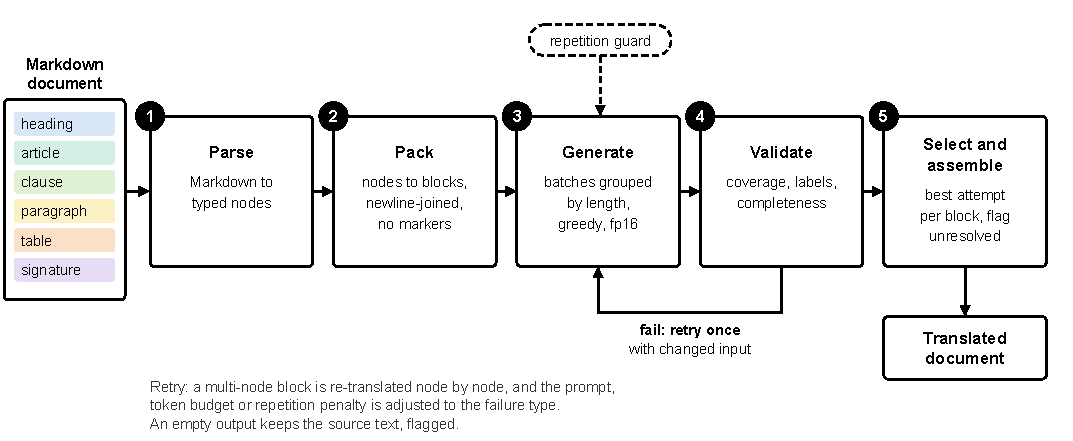
\includegraphics[width=\textwidth]{fig2.pdf}
\caption{Structured translation with one selective recovery round.}
\label{fig:pipeline}
\end{figure*}

\textbf{Parsing and grouping.} A rule-based parser extracts headings, articles, clauses, prose, table cells and signatures while preserving a lossless partition of the raw Markdown. We call each parsed element a \emph{node}; a \emph{unit} is one generation request, which may hold several nodes, and a \emph{prose block} is a unit of coalesced adjacent prose. Adjacent prose of the same scope is coalesced with newline separators and no explicit markers. New articles and higher-level sections create boundaries. Packing targets 768 source tokens or eight nodes, closing at a full-stop boundary; these are soft thresholds to avoid cutting sentences. Tables and signatures use separate handling.

\textbf{Validation.} Hard failures include empty/unmappable outputs, missing EOS, lost protected headings/labels, multiline table-cell outputs and severe repetition. Number mismatches, suspicious length ratios, possible untranslated text and modal/negation discrepancies are warnings, not proofs of semantic errors. Multi-node newline units require one non-empty output line per node; coalesced prose blocks permit internal reflow and retain protected member labels. These checks detect structural failures but cannot guarantee semantic completeness.

\textbf{Recovery and selection.} One recovery round splits failed units into smaller sentence-preserving pieces, targeting 256 source tokens. Failed multi-node newline units are retried independently. Recovery can increase the directional output allowance and applies a 1.15 repetition penalty after loops. Selection favours fewer hard failures, retaining the first pass on ties; complete alternative node outputs can fill gaps. Remaining partial outputs are flagged, and empty translations fall back to source text with a warning.

\textbf{Illustrative example.} An article heading and its clauses ``1.'' and ``2.'' can share a prose block. If the translation drops the protected label ``2.'', validation triggers recovery on smaller, sentence-preserving pieces. Changed line breaks alone do not fail a coalesced prose block, since the check targets structure rather than meaning.

\textbf{Decoding, batching and repetition guard.} Generation is greedy in fp16, with penalty 1.0 on the first pass. Length buckets reduce padding, and a calibration run on the T4 sets the batch size to eight. Every 32 steps after at least 64 generated tokens, a GPU detector examines the last 512 generated tokens. It stops exact consecutive suffix cycles of period 4--64 tokens with at least six repeats covering at least 64 tokens, except patterns repeated at least as often in the input prompt. Tables, signatures and EOS-finished sequences are exempt. Stopped outputs enter validation and bounded recovery; repeated text is not deleted. With $s$ source tokens, the target allowance is
\begin{equation}
b(s)=\max(256,\lceil a s\rceil+128),
\label{eq:budget}
\end{equation}
where $a=1.25$ for first-pass \vien{} prose and $a=2.5$ for \envi{}, protected tables/signatures and full-budget recovery. The actual allowance is bounded by prompt length, a 128-token margin and the sequence limit: normally 8,192 tokens, with a 16,384-token ceiling when preserving a whole sentence requires it.

\begin{table*}[t]
\centering
\begin{tabular}{llcccc}
\toprule
 & & \multicolumn{2}{c}{\envi{}} & \multicolumn{2}{c}{\vien{}} \\
\cmidrule(lr){3-4}\cmidrule(lr){5-6}
Model & System & BLEU & chrF & BLEU & chrF \\
\midrule
Hy-MT2-1.8B & (1) Base, no pipeline & $36.53 \pm 0.02$ & 64.78 & $28.87 \pm 0.04$ & 68.26 \\
 & (2) Base + pipeline & 39.96 & 65.43 & 30.27 & 68.89 \\
 & (3) Fine-tuned + pipeline & \textbf{70.87} & \textbf{84.48} & \textbf{47.44} & \textbf{79.50} \\
\midrule
Index-Translate-2B & (1) Base, no pipeline & 43.96 & 68.74 & 31.22 & 70.55 \\
 & (2) Base + pipeline & 45.49 & 69.26 & 32.38 & 71.15 \\
 & (3) Fine-tuned + pipeline & 62.59 & 78.89 & 41.76 & 76.48 \\
\bottomrule
\end{tabular}
\caption{Results on the public test set, 50 documents per direction. In row (1), Hy-MT2 translates paragraph by paragraph with sampling following its model card, and the value is the mean $\pm$ standard deviation over three seeds. Index uses greedy decoding, so the two (1) rows are not directly comparable.}
\label{tab:main}
\end{table*}

\section{Experiments}\label{sec:experiments}
\subsection{Experimental Setup}
\textbf{Data.} Following the task's recommendation to select systems on the public test set~\cite{vlsp2026}, we report local results on its 50 document pairs in both directions; official private-test scores are not included.

\textbf{Fine-tuning.} For a frozen projection $W_0\in\mathbb{R}^{d\times k}$, LoRA learns $B\in\mathbb{R}^{d\times r}$ and $A\in\mathbb{R}^{r\times k}$:
\begin{equation}
W=W_0+\frac{\alpha}{r}BA.
\label{eq:lora}
\end{equation}
Hy-MT2 uses $r=64$, $\alpha=128$ and dropout 0.05 on q, k, v, o, gate, up and down projections: 77.6 million trainable parameters (Appendix~\ref{app:lora}). The sample-length check uses the complete model-specific chat template:
\begin{equation}
n(x,y)=\big|\operatorname{Tok}(\operatorname{Chat}(P(x),y))\big|.
\label{eq:len}
\end{equation}
Here $P(x)$ includes the instruction and optional terminology hints; the chat renderer includes all special tokens. Hy-MT2 rejects samples above 3,072 tokens rather than truncating them; none were dropped in the final run.

\textbf{Inference.} Each direction runs on one Kaggle T4 with Transformers, greedy fp16 decoding, batch size eight and one recovery round. LoRA weights are merged into the base model before inference, so the deployed model has 1.79B parameters, below the 3B limit; inference runs locally without external APIs. Appendix~\ref{app:hyper} lists the remaining settings.

\textbf{Metrics.} We use case-sensitive SacreBLEU with tokenizer 13a~\cite{post2018sacrebleu} and chrF with character order six, word order zero and $\beta=2$~\cite{popovic2015chrf}. Each complete Markdown document is one metric segment: 50 hypothesis--reference pairs per direction, without line splitting. Scores aggregate corpus statistics, rather than averaging document scores. Lexical and Unicode content is retained; Windows CRLF is restored to LF. BLEU on the reported 0--100 scale is~\cite{papineni2002bleu}
\begin{equation}
\begin{aligned}
\mathrm{BLEU}&=100\,\mathrm{BP}\exp\Big(\tfrac14\sum_{n=1}^{4}\log p_n\Big),\\
\mathrm{BP}&=\min(1,e^{1-r_{\mathrm{ref}}/c}),
\end{aligned}
\label{eq:bleu}
\end{equation}
where $p_n$ are corpus modified precisions in $[0,1]$, and $c,r_{\mathrm{ref}}$ are hypothesis/reference token counts. SacreBLEU handles zero-match and empty-output cases. Likewise,
\begin{equation}
\mathrm{chrF}_\beta=100\,\frac{(1+\beta^2)\mathrm{chrP}\,\mathrm{chrR}}{\beta^2\mathrm{chrP}+\mathrm{chrR}},
\label{eq:chrf}
\end{equation}
where precision and recall are averaged over effective character $n$-gram orders and expressed as fractions. Whitespace is excluded under the default chrF configuration; a zero denominator yields zero.

Paired bootstrap resampling~\cite{koehn2004significance} draws 50 documents with replacement and recomputes corpus scores on the same sampled documents for both systems:
\begin{equation}
\Delta_b=\mathrm{BLEU}_b(S_2)-\mathrm{BLEU}_b(S_1).
\label{eq:boot}
\end{equation}
The 2.5th and 97.5th percentiles define a 95\% interval. We use seed 42 and 1,000 paired resamples for grouping comparisons, plus 2,000 resamples for final-system BLEU intervals. The latter quantify document-sampling uncertainty, not an improvement over a baseline or variability across training seeds.

\begin{table}[t]
\centering
\footnotesize
\resizebox{\columnwidth}{!}{%
\begin{tabular}{lcccc}
\toprule
 & \multicolumn{2}{c}{\envi{}} & \multicolumn{2}{c}{\vien{}} \\
\cmidrule(lr){2-3}\cmidrule(lr){4-5}
Design & BLEU & chrF & BLEU & chrF \\
\midrule
A: markers & 68.70 & 83.24 & 46.37 & 79.01 \\
B: no markers & \textbf{68.90} & \textbf{83.39} & \textbf{46.62} & \textbf{79.17} \\
C: separate & 67.69 & 82.64 & 45.23 & 78.23 \\
\bottomrule
\end{tabular}}
\caption{Two grouping designs and per-node translation on a model fine-tuned on about 53.5 thousand training rows, in the first version of the pipeline. Settings: repetition penalty 1.05, batch size 4, one run per design.}
\label{tab:design}
\end{table}

\begin{table}[t]
\centering
\footnotesize
\resizebox{\columnwidth}{!}{%
\begin{tabular}{lcccc}
\toprule
 & \multicolumn{2}{c}{Time (s)} & \multicolumn{2}{c}{GPU alloc. (GB)} \\
\cmidrule(lr){2-3}\cmidrule(lr){4-5}
System & \envi{} & \vien{} & \envi{} & \vien{} \\
\midrule
(1) & $\sim$4.0k & $\sim$4.1k & 5.41 & 4.90 \\
(2) & 8,111 & 5,326 & 5.34 & 5.15 \\
(3) & 7,229 & 4,871 & 4.96 & 5.25 \\
\bottomrule
\end{tabular}}
\caption{Hy-MT2 running time and peak allocated GPU memory per direction on one T4 (decimal GB). Systems follow Table~\ref{tab:main}; (1) is per seed.}
\label{tab:cost}
\end{table}

\subsection{Results}
Table~\ref{tab:main} compares (1) paragraph-wise base-model translation, (2) the base model with the pipeline and (3) the fine-tuned model with the pipeline. For Hy-MT2, (1) uses sampling and (2)--(3) use greedy decoding, so (1)--(2) changes both decoding and pipeline. The (2)--(3) comparison measures fine-tuning with the pipeline fixed, without separating the effects of cleaning and augmentation.

\textbf{Pipeline and fine-tuning.} For Index, where decoding is fixed, the pipeline adds 1.53/1.16 BLEU; for Hy-MT2 the gain also reflects the change from sampling to greedy decoding. Fine-tuning yields the largest observed gain: Hy-MT2 improves from 39.96 to 70.87 BLEU for \envi{} and from 30.27 to 47.44 for \vien{}. Index shows the same trend. The final-system BLEU intervals are [65.68, 74.24] for \envi{} and [42.30, 50.99] for \vien{}. Scores in opposite directions are not directly comparable, so we report them separately.

\textbf{Model choice.} Index has higher base scores, including row (2), where both models use greedy decoding with the pipeline. After fine-tuning, however, Hy-MT2 scores higher in both directions and is selected for submission. The remaining analyses use Hy-MT2.

\textbf{Pipeline design.} An earlier checkpoint trained on approximately 53.5k rows compares grouped translation with markers (A), grouping without markers (B) and separate node requests (C), as shown in Table~\ref{tab:design}. Both grouped variants score higher than C. B exceeds A by 0.20/0.25 BLEU for \envi{}/\vien{} and avoids marker handling; it motivates the final prose-block design. Paired 95\% intervals for B$-$A are [0.05, 0.37] (\envi{}) and [$-$0.06, 0.68] (\vien{}); B$-$C intervals are [0.75, 1.52] and [0.61, 2.20]. Thus grouping improves on separate requests in both directions, whereas the marker-free advantage over A is uncertain for \vien{}. This earlier-pipeline experiment does not isolate every final-system component.

\subsection{Cost}
Table~\ref{tab:cost} reports full-public-set inference cost. The fine-tuned pipeline takes 7,229~s (2.0~h) for \envi{} and 4,871~s (1.4~h) for \vien{}, with 4.96/5.25~GB peak allocated GPU memory (decimal GB), measured by PyTorch; this excludes the CUDA context and allocator cache, so process-level usage is higher. Timing excludes model loading and calibration. Recovery re-translates 138 of 2,899 \envi{} units (4.76\%) and 326 of 3,086 \vien{} units (10.56\%), splitting them into 836 and 1,443 smaller requests. Earlier grouping runs took 4.6/2.9~h; their different checkpoint and pipeline preclude isolating one optimisation.

Unresolved units total 26/2,899 (0.90\%) across 11 documents for \envi{}: 25 have protected-label failures and one a protected-heading failure. For \vien{}, 208/3,086 (6.74\%) across 29 documents include 198 with protected-block-label failures, 11 with line-count mismatches, three with inline-label failures and one with a heading failure; categories overlap. Final diagnostics record no unresolved empty nodes, source fallbacks, missing-EOS or repetition hard failures in either direction. Thus these rates measure remaining structural-check failures, not measured omission rates; partial content and semantic omissions still require direct translation review.

\section{Limitations and Discussion}\label{sec:limitations}
Systems are selected on the public set following the task guidance, so the reported scores describe development performance rather than an independent evaluation. Validation-loss monitoring uses the internal held-out split. We report no official private-test rankings, no legal-accuracy or terminology scores and no neural or LLM-based metrics, although the official evaluation includes them.

Structural validation cannot establish semantic fidelity or document-wide terminology consistency, and unresolved blocks can retain partial or untranslated text. Further evaluation should examine omissions, obligations, negation and terminology with domain experts. Additional ablations could separate cleaning/augmentation, decoding, grouping and recovery; inference-time glossary hints remain untested systematically. Tone-mark normalisation follows the older placement used in most training text; public-test references using the newer placement are not normalised, which can lower \envi{} scores on those documents.

\begin{samepage}
\section{Conclusion}
Our VLSP 2026 submission combines legal-domain LoRA adaptation of Hy-MT2-1.8B with structured Markdown translation and selective recovery. It reaches 70.87/47.44 public-test BLEU for \envi{}/\vien{} with approximately 5~GB peak allocated GPU memory and 2.0/1.4~h per direction on a T4. These development results motivate a practical small-model pipeline, while independent legal-accuracy and generalisation evaluation remains necessary.

\end{samepage}

\bibliography{references}

\appendix
\section{Prompts}\label{app:prompts}
For Hy-MT2, the user-turn inference prompt is:
\begin{quote}\small\ttfamily\raggedright
Translate the following text into \{tgt\}. Note that you should only output the translated result without any additional explanation:\par\medskip
\{src\}
\end{quote}
Here \texttt{tgt} is English or Vietnamese. Terminology training prompts prepend \texttt{Reference the following translations:}, newline-separated \texttt{source translates to target} pairs and a blank line; the instruction uses \texttt{must ONLY} instead of \texttt{should only}. Inference supplies neither glossary hints nor target history. Index uses its Chinese translation-only instruction with thinking disabled.

\section{Hyperparameters}\label{app:hyper}
Table~\ref{tab:hyper} records the Hy-MT2 training and submitted inference configuration. Hy-MT2 trains first on approximately 53.5k rows and then on 82,203 rows. Base revisions are \texttt{9a341cd1b679} (Hy-MT2) and \texttt{a516854233b1} (Index); the final Hy-MT2 adapter SHA-256 starts with \texttt{30b5fc68a31c}.

\noindent\begin{minipage}{\columnwidth}
\centering\small
\begin{tabularx}{\columnwidth}{@{}lX@{}}
\toprule
Setting & Hy-MT2 value \\
\midrule
LoRA & $r=64$, $\alpha=128$, dropout 0.05; q/k/v/o and gate/up/down \\
Schedule & 1 epoch/pass; LR $2\!\times\!10^{-4}$ then $5\!\times\!10^{-5}$; second pass: 2,569 steps, 25 warm-up steps, cosine decay to 10\% \\
Training & fp16 DDP, two T4s; batch $1\!\times\!16\!\times\!2=32$; max length 3,072; weight decay 0; clipping 1; seed 42 \\
Decoding & greedy fp16; batch 8; penalty 1.0, or 1.15 after a loop; one recovery round \\
Packing & prose 768 tokens/8 nodes (soft); tables 384/16; signatures 128; recovery 256 tokens \\
Budget & Eq.~\eqref{eq:budget}; context 8,192, sentence ceiling 16,384; margin 128 \\
Repetition & GPU check every 32 generated steps, minimum 64 tokens \\
Runtime & torch 2.11.0+cu128; Transformers 5.8.1; tokenizers 0.22.2 \\
Scoring & SacreBLEU 2.6.0; BLEU: 13a, mixed case, exponential smoothing; chrF: order 6, $\beta=2$, word order 0, no whitespace \\
\bottomrule
\end{tabularx}
\captionof{table}{Hy-MT2 training and inference settings. Runtime versions refer to the submission run.}
\label{tab:hyper}
\end{minipage}

\section{Computing the Number of LoRA Parameters}\label{app:lora}
Each adapted projection contributes $r(d_{\mathrm{in}}+d_{\mathrm{out}})$ weights. For $L$ identical layers and projection set $\mathcal{M}$,
\begin{equation}
N_{\mathrm{LoRA}}=L\sum_{m\in\mathcal{M}}r(d_{\mathrm{in}}^{(m)}+d_{\mathrm{out}}^{(m)}),
\end{equation}
\begin{equation}
\rho=\frac{N_{\mathrm{LoRA}}}{N_{\mathrm{base}}+N_{\mathrm{LoRA}}}.
\end{equation}
For Hy-MT2, $L=32$, $r=64$; q/o shapes are $2048\!\times\!2048$, k/v $512\!\times\!2048$, gate/up $6144\!\times\!2048$, and down $2048\!\times\!6144$. Thus $N_{\mathrm{LoRA}}=77{,}594{,}624$ and $\rho=77{,}594{,}624/(1{,}791{,}080{,}448+77{,}594{,}624)\approx4.15\%$. Relative to frozen base weights alone, the ratio is 4.33\%.

\end{document}
